\documentclass[
  11pt,
  fleqn
]{article}
% [fleqn] left-aligns all equations

% fonts

\usepackage[T1]{fontenc} % Apparently this
% https://tex.stackexchange.com/questions/287312/font-not-loadable-metric-data-not-found-or-bad
\usepackage[full]{textcomp}
\usepackage[final,expansion=alltext,nopatch=footnote]{microtype}
\usepackage{csquotes} % suppress warning from `babel`
\usepackage[english]{babel}
\usepackage[fleqn]{mathtools}
\usepackage[cal=boondoxo]{mathalpha} % mathcal

\usepackage{amsthm} % gives proof environment:
% https://www.overleaf.com/learn/latex/Theorems_and_proofs

\usepackage{newtxtext}
% \usepackage{txfonts} % See
% https://tex.stackexchange.com/questions/444243/symbols-not-showing-up

% These need to be after newtxtext
\usepackage[varqu,varl]{inconsolata} % sans serif typewriter
% \usepackage{cabin} % sans serif - ugly

\usepackage[bigdelims,vvarbb]{newtxmath} % bb from STIX % "should be
% loaded AFTER the text font" -
% https://mirrors.mit.edu/CTAN/fonts/newtx/doc/newtxdoc.pdf

% geometry of the page

\usepackage[
  % top=1in,
  % bottom=1in,
  % left=1in,
  % right=1in
]{geometry}

% paragraph spacing

\setlength{\parindent}{0pt}
\setlength{\parskip}{1.5ex plus 0.4ex minus 0.2ex}

% useful packages

% \usepackage{natbib} % incompatible with BibLaTeX
\usepackage{epsfig}
\usepackage{url}
\usepackage{bm}
\usepackage{blindtext}

% Leon additions

\usepackage{enumitem} % allows for enumerate[resume]

\usepackage{booktabs}

\usepackage[
  style=authoryear-comp,
  natbib=true,
  % refsection=chapter,
  url=false,
  doi=true,
  isbn=false,
  date=year %
  % https://tex.stackexchange.com/questions/55780/disable-month-in-biblatex-bibliography
]{biblatex} % natbib=true allows \citep
% Clear "visited on"
% https://tex.stackexchange.com/questions/400384/how-to-disable-biblatex-showing-visited-on-on-the-references
\AtEveryBibitem{
  \clearfield{urlyear}
  \clearfield{urlmonth}
  \clearfield{eprint} % remove PMID %
  % https://tex.stackexchange.com/questions/250784/removing-eprint-and-eprinttype-in-citation-notes
}

\usepackage{graphicx}
% ensures figures stay in their section
% https://tex.stackexchange.com/questions/279/how-do-i-ensure-that-figures-appear-in-the-section-theyre-associated-with
\usepackage[section]{placeins}

% Section formatting using titlesec
\usepackage{titlesec}
\titleformat*{\section}{\singlespacing\sffamily\Large}
\titleformat*{\subsection}{\singlespacing\sffamily\large}
% \titleformat*{\subsubsection}{\itshape}
\titleformat*{\paragraph}{\itshape}
\titleformat{\chapter}{\singlespacing\sffamily\Huge}{{\thechapter}}{1em}{}

% center figures by default
\makeatletter
\g@addto@macro\@floatboxreset\centering
\makeatother
% italic figure captions
\usepackage[format=plain,
  textfont=it,
]{caption}

% simple TO DO and comment macros
\usepackage[
  % https://tex.stackexchange.com/questions/4503/how-do-i-specify-color-in-rgb-using-hypersetup-in-hyperref
  dvipsnames,svgnames,x11names
]{xcolor}
\newcommand\todo[1]{\textcolor{orange}{[#1]}}% simple TO DO macro
\newcommand\comment[1]{\textcolor{red}{[#1]}}

\usepackage{url}
\usepackage[
  hidelinks,
  pdfa % Required for valid pdf/a output:
  % https://tex.stackexchange.com/questions/431022/pdf-a-validation-problem-the-f-key-is-missing
]{hyperref}
\hypersetup{
  % colorlinks,
  % linkcolor=RoyalBlue4,
  % citecolor=PaleVioletRed4,
  % urlcolor=Firebrick4
}

\newcommand{\indsim}{\overset{\mathrm{ind}}{\sim}}
% https://tex.stackexchange.com/questions/60545/should-i-mathrm-the-d-in-my-integrals
\newcommand*\diff{\mathop{}\!\mathrm{d}}
\newcommand*\Diff[1]{\mathop{}\!\mathrm{d^#1}}
\newcommand{\e}{\mathrm{e}}
\newcommand{\E}{\mathrm{E}}
\renewcommand{\P}{\mathrm{P}}
\newcommand{\N}{\mathrm{N}}
\newcommand{\diag}{\mathrm{diag}}
\newcommand{\ave}{\mathrm{ave}}
\newcommand{\Var}{\mathrm{Var}}
\newcommand{\Cov}{\mathrm{Cov}}
\newcommand{\cov}{\mathrm{cov}}
\newcommand{\sd}{\mathrm{sd}}
\newcommand{\var}{\mathrm{var}}
\newcommand{\corr}{\mathrm{corr}}
\renewcommand\vec{\boldsymbol}

% Overlap-specific
\newcommand{\rank}{R}
\newcommand{\rmax}{m}
\newcommand{\rgap}{r^\text{gap}}
\newcommand{\Ngap}{N_1^\text{gap}}
\newcommand{\pigap}{\pi_1^\text{gap}}

% For appearance of block matrices
% https://tex.stackexchange.com/questions/495903/horizontal-and-vertical-lines-in-pmatrix
\renewcommand{\arraystretch}{1.5}

% Theorem-type environments
\newtheorem{definition}{Definition}[section]
\newtheorem{result}[definition]{Result}
\newtheorem{claim}[definition]{Claim}

% From Datta template
% https://github.com/bibekanandadatta/JHU-Dissertation-Template

\usepackage{setspace}                         % sets space between lines

%%%% JH Library requirement (DO NOT CHANGE)
\def\GlobalMargin{1.0in}                      % margin on all sides
% \def\PrintingOffset{0.5in}                  % additional left
% margin for the printed copy
\def\PrintingOffset{0.0in}
\def\MainTextSpacing{\singlespacing}        % double-spaced main text
% \def\MainTextSpacing{}
\def\CaptionStretch{1.1}                    % to match 2x spacing
% \def\CaptionStretch{1.0}

\captionsetup{font={stretch=\CaptionStretch}}

\geometry{
  letterpaper,
  margin=\GlobalMargin,
  bindingoffset=\PrintingOffset,
  nomarginpar,
  % includehead,
  % headheight=\HeaderHeight,
  % headsep=\HeaderSpace,
  includefoot,
  heightrounded
}

%%%% BIBLIOGRAPHY ITEMS
\def\BibTextSpacing{\onehalfspacing}         % single-spaced bibliography
% \def\BibTextSpacing{\singlespacing}         % single-spaced bibliography
\def\BibItemSpacing{\baselineskip}          % spacing between
% bibliographic items in reference

%%%% UNNUMBERED CHAPTERS, SECTION, and SUBSECTION COMMAND for ADDING to TOC
%% removes the 'Chapter #' title while keeping it listed in the TOC
\newcommand\chap[1]{%
  \chapter*{#1}%
  \markboth{#1}{}
\addcontentsline{toc}{chapter}{#1}}

%% removes the 'Section #' title while keeping it listed in the TOC
\newcommand\sect[1]{%
  \phantomsection
  \section*{#1}%
\addcontentsline{toc}{section}{#1}}

%% removes the 'Subsection #' title while keeping it listed in the TOC
\newcommand\subsect[1]{%
  \phantomsection
  \subsection*{#1}%
\addcontentsline{toc}{subsection}{#1}}

%% removes the 'Subsubsection #' title while keeping it listed in the TOC
\newcommand\subsubsect[1]{%
  \phantomsection
  \subsubsection*{#1}%
\addcontentsline{toc}{subsubsection}{#1}}

% Correct matrix for double spacing
% https://tex.stackexchange.com/questions/137004/matrix-within-equation/137009#137009
\makeatletter
\def\env@matrix{\hskip -\arraycolsep
  \let\@ifnextchar\new@ifnextchar
  \linespread{1}\selectfont
  \renewcommand{\arraystretch}{1.2}%
\array{*\c@MaxMatrixCols c}}
\makeatother

% Footnotes must be 2 points less than main text but larger than 8pt
\usepackage{footmisc}
\renewcommand{\footnotesize}{\fontsize{9pt}{11pt}\selectfont}

% For including CV
\usepackage{pdfpages}

% Generate PDF/A (archival format)
% https://webpages.tuni.fi/latex/pdfa-guide.pdf
\usepackage[a-1b,mathxmp]{pdfx}

\usepackage[
  nottoc % Don't include TOC in TOC
]{tocbibind}

% Redefine `abstract`s so they can be at the start of each chapter
% don't cause the page numbering to reset
% https://tex.stackexchange.com/a/4857
\newenvironment{myAbstract}{
  \rightskip.5in
  \leftskip.5in
  % \itshape
}{}

% For writing/planning purposes: show paragraph level in TOC
\setcounter{secnumdepth}{3}

\addbibresource{references.bib}
\graphicspath{{fig/}}

\title{Choosing ordinal effect measures for clinical trials}
\author{Leon Di Stefano + Ordinal
Working Group}
\date{\today}

\begin{document}

\maketitle

\tableofcontents
\newpage

\section{Introduction}

\section{Desiderata for ordinal effect measures}

Effect measures compare distributions of outcomes across groups
under different interventions or exposures.

We generally seek effect measures that
\begin{enumerate}
  \item correspond most directly to patient benefit/harm
  \item are easy to interpret and to translate into practical recommendations
  \item can be incorporated into statistical models where required
  \item are easy to generalize or ``transport'' across contexts or settings
\end{enumerate}

Key references for ordinal effect measures:
\citet{agrestiMeasuresNominalOrdinalAssociation1981,agrestiOrdinalProbabilityEffect2017,
agrestiSimpleWaysInterpret2018}.

We want to compare two or more distributions over ordinal
outcomes with a single number. We want to compare \emph{two} distributions
when when there are two interventions (call them control and
experimental). But in multi-arm studies or when e.g. adjusting for
covariates, it may become important to compare more than 2 groups
(see the transitivity in Section \ref{sec:comparing}).

Summarizing the comparison between two distributions with a single
number represents a loss of information. Let's say the
outcome has $C$ categories. Then the distribution in each
arm is non-redundantly specified by $C-1$ numbers (for the first
  $C-1$ probabilities,
  or cumulative logits, or stopping ratio logits--reflecting the
sum-to-1 constraint on probability distributions) and so the
\emph{difference} between the distributions is also non-redundantly specified by
$C-1$ numbers (for example the differences between the cumulative
  logits, or logit stopping probabilities -- these latter numbers are
unconstrained).

Since an effect measure thus represents a way to collapse these $C-1$
numbers into one, it must lose information.

Truly ordinal effect measures depend only on the ordinal structure of
the outcomes, rather than, for example, a particular numeric coding
(e.g. difference in mean levels). This is adding
information that is not present in the ordinal structure.

\section{Model-based effect measures}

\begin{figure}
  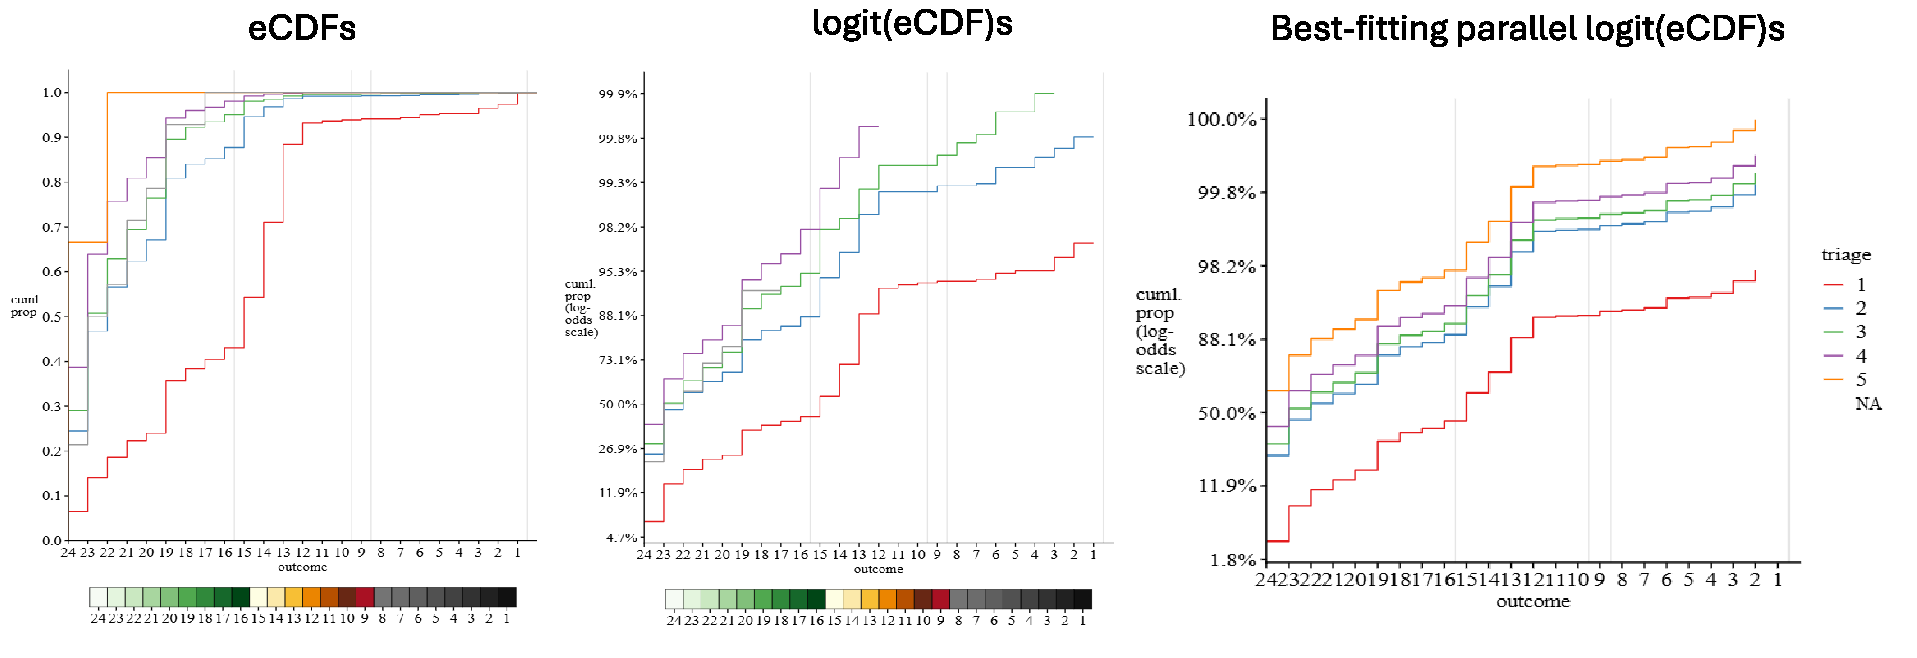
\includegraphics[width=7in]{illustrating_common_or.pdf}
  \caption{The common odds ratio, a model-based effect measure, comes
    from the best-fitting parallel curves to the logit transformed
    empirical cumulative distribution. \textbf{Ideally would illustrate
      using toy bar charts as above, with only 2 groups? Although it's a
  strength that model-based measures can compare multiple groups.}}
  \label{fig:illustrating_or}
\end{figure}

\begin{itemize}
  \item
    common odds ratio (or e.g. probit analogue; there are versions of
    this for any cumulative link)
  \item Others: common stopping ratio (hazard ratio is an example
    with implicitly ordinal time) or common continuation
    ratio;
    see
    \citet{burknerOrdinalRegressionModels2019,agrestiAnalysisOrdinalCategorical2010}
    for more.
\end{itemize}

What they have in common: the effect measure is a byproduct of fitting a model
to the data.
The model assumes that a certain \emph{pattern} is present in the outcome
distributions across groups. If the pattern (approximately) holds,
then the differences in
distributions can (approximately) be described by a single number.
See Figure \ref{fig:illustrating_or} for an illustration
for the common odds ratio.

Usually model-based effect measures can put multiple groups on a
common ``scale''. This is important when adjusting for prognostic
factors, for example.
A proportional odds model does this with the scale defined by a
common set of cutpoints
or ``intercepts''.
Figure \ref{fig:illustrating_or} illustrates this; the pattern
assumed to hold is
that the logit-transformed eCDFs in each group are parallel.

\section{Model-free or nonparametric effect measures}

These are not based on a model (assumed pattern in the differences
between outcome distributions).

\subsection{Effect measures based on ``independent pairs'' or
``win'' constructions}

\begin{figure}
  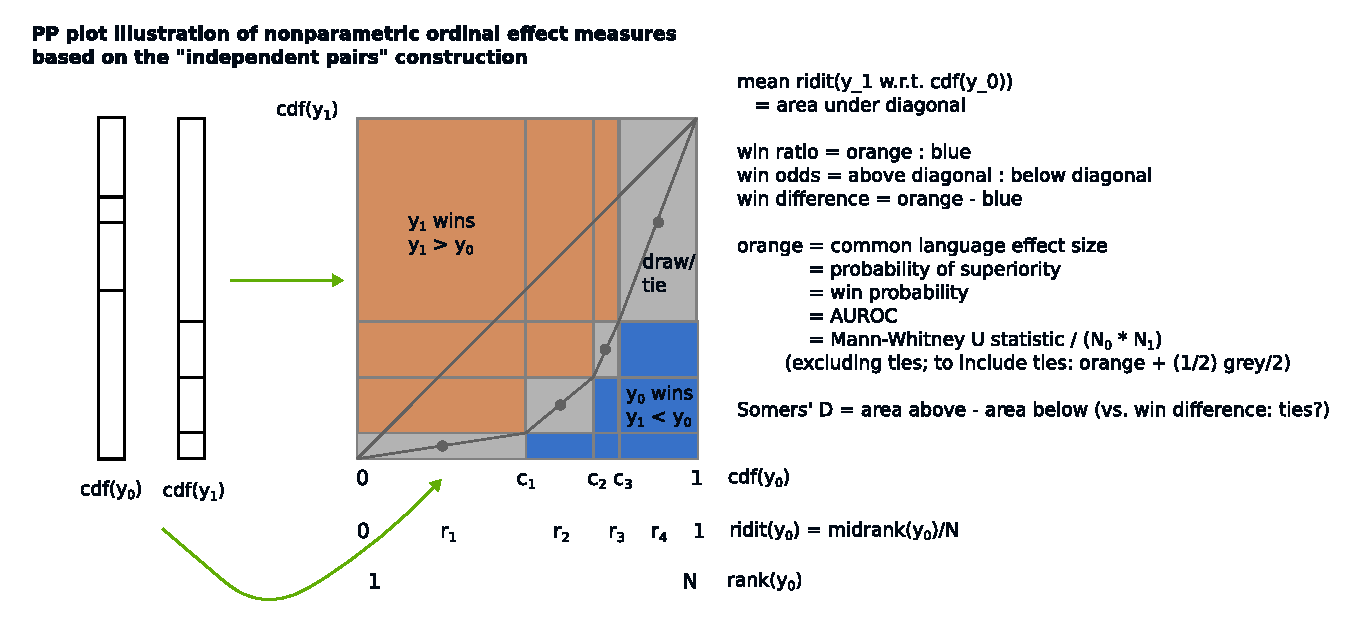
\includegraphics[width=7in]{effect_measures_pp_plot.pdf}
  \caption{\textbf{Illustrating independent pairwise comparison-based effect
    measures using a PP-plot or ROC curve.}
    The $x$ axis shows the
    cumulative distribution function (CDF) of $y$ under the control
    intervention; the $y$ axis shows the CDF under the experimental
    intervention. The grey
    curve (\emph{P-P} curve) shows how the CDFs vary with one
    another; a curve below the diagonal indicates that the CDF of $y$
    under the experimental treatment is lower than the CDF of $y$
    under control, and therefore that $y$ is stochastically greater
    under the experimental treatment. Areas in the plot correspond to
    probabilities under
    the ``independent pairwise comparisons'' construction: the orange
    area corresponds to the win probability (or probabilistic index,
    probability of superiority, common language effect size) in favor
    of the experimental treatment. The ratio of orange and blue areas
    is the win ratio, and if the grey area -- corresponding to tied
    pairs under independent draws -- is allocated equally to orange
    and blue, the ratio of areas corresponds to the win odds.
    Adapted from
  \citet{smithsonReceiverOperatingCharacteristic2023}.}
  \label{fig:illustrating_pairwise_comparisons}
\end{figure}

Probabilistic index, probability of
superiority, common language effect size, win ratio, win odds, etc.
These predate win ratio and
DOOR methods and have been reinvented many times
\citep[e.g.][p.~14]{agrestiAnalysisOrdinalCategorical2010}.

They are all be based on the ``\emph{pairs construction}'',
where we imagine independently sampling patients from the control and
treatment groups and considering ``wins'' ``ties'' and ``losses''
(corresponding to concordant and discordant pairs and ties in $y$
respectively). See Figure \ref{fig:illustrating_pairwise_comparisons}
for an illustration.

They can
also be \emph{estimated from data} using pairs of patients, but this
is not essential and they could also be estimated by fitting a
proportional odds model, for example (though they would not be a
simple function of a coefficient).

They generalize binary effect measures and can themselves be
generalized beyond comparing two groups to the situation where $x$ is
also ordinal.

\subsection{Effects based on the pairs constructions do not measure
individual-level effects}

Pair-construction or win methods have a subtle issue of interpretation.

The win probability is \emph{not} the probability that a given
individual's outcome under the experimental treatment is better than
what would be obtained under the control treatment.

Rather is the probability that an individual drawn at random
from the experimental group has a better outcome than a \emph{different}
individual drawn at random from the control group.

The issue is similar to that for \emph{p}-values, which is subtly
different from -- and often confused for -- ``the thing we want''
(namely the posterior probability of the null hypothesis).

Relatedly, I believe that \emph{win probabilities and win
differences, unlike risks and risk differences, are non-collapsible}
in the sense that the average of win probabilities (or differences)
across strata is not necessarily equal to the win probability (or
difference) in the unstratified population.

\begin{figure}
  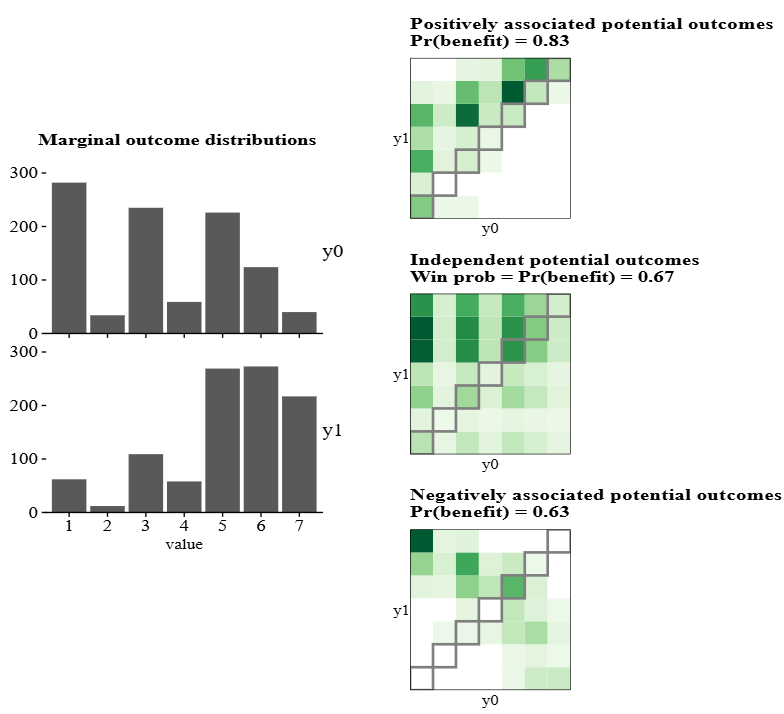
\includegraphics[width=5in]{po_association_discrete.png}
  \caption{\textbf{Effect measures based on the ``independent pairs''
    construction do not refer to individual-level benefit/harm.}
    Left: two ordinal outcome distributions. Right: different
    possible joint distributions of potential outcomes with marginals
    corresponding to the distributions on the left.
    The ``probability of benefit'' -- probability that a randomly
    selected \emph{individual} does better under the experimental
    intervention than the control intervention -- depends on the
    joint distribution and is higher when potential outcomes are
    positively associated. The win probability is the probability of
    benefit when the potential outcomes are independent (or the
      probability that experimental intervention ``beats'' control in a
    random \emph{pair} of individuals).
  }
  \label{fig:pairwise_and_pos_discrete}
\end{figure}
\begin{figure}
  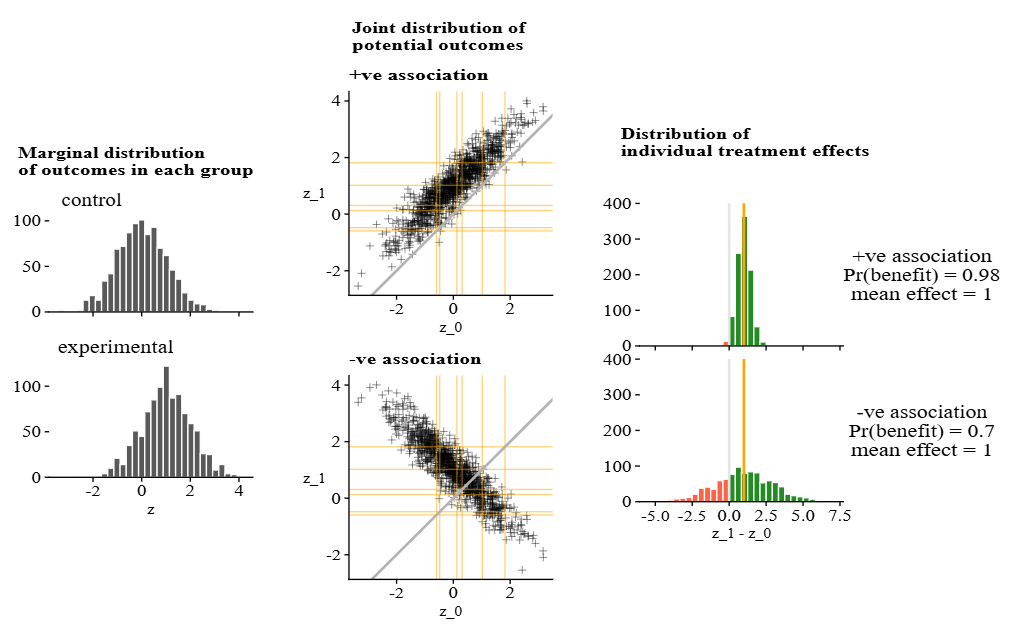
\includegraphics[width=7in]{po_association_continuous.png}
  \caption{\textbf{Effect measures based on the ``independent pairs''
    construction do not refer to individual-level benefit/harm.}
    This figure is meant to illustrate the same point as Figure
    \ref{fig:pairwise_and_pos_discrete}, but with
    continuous outcomes. They make things easier because it's
    possible to plot the
    \emph{distribution} of individual-level treatment effects. (By
      contrast, with ordinal outcomes there's no natural notion of the
      difference between two levels of the scale and hence no compact way to
    represent individual effects.) The orange criss-crosses are
    cutpoint used to generate the data in Figure
    \ref{fig:pairwise_and_pos_discrete}.
    \todo{Ways to make the two plots more parallel: have green and
      red (or blue and red) in the discrete heatmaps too; include an
    independence case for the continuous outcomes.}
  }
  \label{fig:pairwise_and_pos_continuous}
\end{figure}

\subsection{Dichotomizing or using more than a single number}

Ways to dichotomize:

\begin{itemize}
  \item Dichotomizing by picking a specific cutpoint,
    e.g. ``hospitalization or
    worse''. This is effectively using a binary outcome, but with the
    ordinal structure used to gain power if fitting a model.
  \item Dichotomizing using quantiles of a reference
    group; for example,
    ``proportion in the treated group with worse outcomes than the
    median outcome under standard care''
\end{itemize}

Ways to use more than a single number to summarize effects:

\begin{itemize}
  \item Plotting cumulative distribution functions or survival functions
  \item Plotting ridits, which compare ordinal distributions using a
    reference group and are closely connected to win probability
    \citep{brossHowUseRidit1958,agrestiAnalysisOrdinalCategorical2010,
      smithsonReceiverOperatingCharacteristic2023,
    jansenRiditAnalysisReview1984}
\end{itemize}

\section{Comparing model-based and nonparametric effect measures}
\label{sec:comparing}

Both of these can be considered ``estimands'', insofar as we consider the
estimand associated with the model-based effect measures to be given by the
best-fitting model in the population.

Two classes of assumption violations for model-based effect measures
are \emph{magnitude}-heterogeneity across cutpoints (for example,
  effect of a treatment on hospital length of stay or worse is larger
  than its effect on
death on the relevant scale) and
\emph{sign}-heterogeneity
across cutpoints (failure of stochastic dominance -- for example,
treatment is beneficial for hospital length of stay, harmful for death).

Nonparametric effect measures may appear to be assumption-free. However

\begin{itemize}
  \item Assumptions don't need to hold exactly for the model-based
    effect measures to make sense
    \begin{itemize}
      \item In particular, if stochastic dominance holds, we can think of
        both model-based and nonparametric effect measures as
        testing the null hypothesis of no effect ``in a specific
        direction''. A weak interpretation of any particular
        effect measure
        is that it supplies this ``direction''.

        For example the Wilcoxon test is
        equivalent to the score test from fitting a proportional odds model;
        the implied ``directions from the null'' are the same.
        Thus fitting a proportional odds model (or any other model) has a
        valid null-testing
        interpretation even if proportional odds doesn't hold.
      \item Under failure of stochastic dominance (``sign
        heterogeneity''), \emph{neither} parametric nor nonparametric
        effect measures make sense, since it doesn't make sense to
        summarize effects by a single number. Need to dig into the
        cutpoint-specific effects.
    \end{itemize}
  \item Model-free methods don't define a common scale for comparing
    more than two interventions. For example, model-free effect
    measures can be \emph{nontransitive}, so it's not clear how to
    use them in $\geq 2$-arm studies.

    That said, when comparing more than two distributions \emph{that
    can be ordered} (i.e. when $x$ as well as $y$ is ordinal),
    Somers' $D$ is a generalization of the win difference, Harrell's
    $c$-index is a generalization of the win probability, and
    \citet{newsonParametersNonparametricStatistics2002} discusses a
    generalization of the win ratio.

  \item Model-based methods allow one to adjust for covariates.

    When additivity approximately holds, this yields a ``best of both
    worlds'' effect measure that is
    personalized (conditional) yet reportable as a single
    number.
\end{itemize}

Harrell critiques \citep{harrellOverviewCompositeOutcome2024,
harrellRareDegenerativeDiseases2024, harrellViewsCompositeOutcome}:
mainly that
win probability etc. are \emph{relative measures}:

\begin{itemize}
  \item Comparable to Cohen's $d$ or $t$-statistic (difference in
    means divided by standard deviation or standard error) rather than
    difference in means: compare: standardized effect size of 0.2 vs.
    difference in means of 10 mmHg
  \item Affected by study inclusion criteria (why? probably needs to
    be fleshed out.)
  \item This may unintentionally make interpreting estimated effect
    sizes for the purposes of both study planning and interpreting results.
\end{itemize}

Another set of critiques are in
\citet{hartmanPitfallsConcordanceIndex2023}. I haven't understood
these yet but the main concern seems to be that more comparable cases
(in terms of baseline risk) are more likely to have ties. So there's
a tradeoff between relevance of the comparisons (conditioning on
similar baseline risk) and informativeness of the comparisons
(avoiding ties/getting clear "wins").

Simulations show a typically very strong association between
[double check] log common odds ratios and log win ratios (both of
which generalize the odds ratio for a binary variable)
\citep{harrellViolationProportionalOdds2020}.

We should distinguish between effect measures used for \emph{design
and decision-making},
for \emph{analysis}, and for
\emph{reporting}. For example it might make most sense to design a
study and define decision rules using a common odds
ratio/proportional odds model, but to
additionally report results using the win probability..
It may make
sense to report the probabilistic index or a
single-cutpoint binary outcome even if the analysis is undertaken using a
proportional odds model. Reporting win statistics based on model fits is
suggested in \todo{one of}
\cite{agrestiOrdinalProbabilityEffect2017,agrestiSimpleWaysInterpret2018}

\section{Conclusion}

\newpage

\printbibliography

\end{document}